\begin{figure}[p]\centering
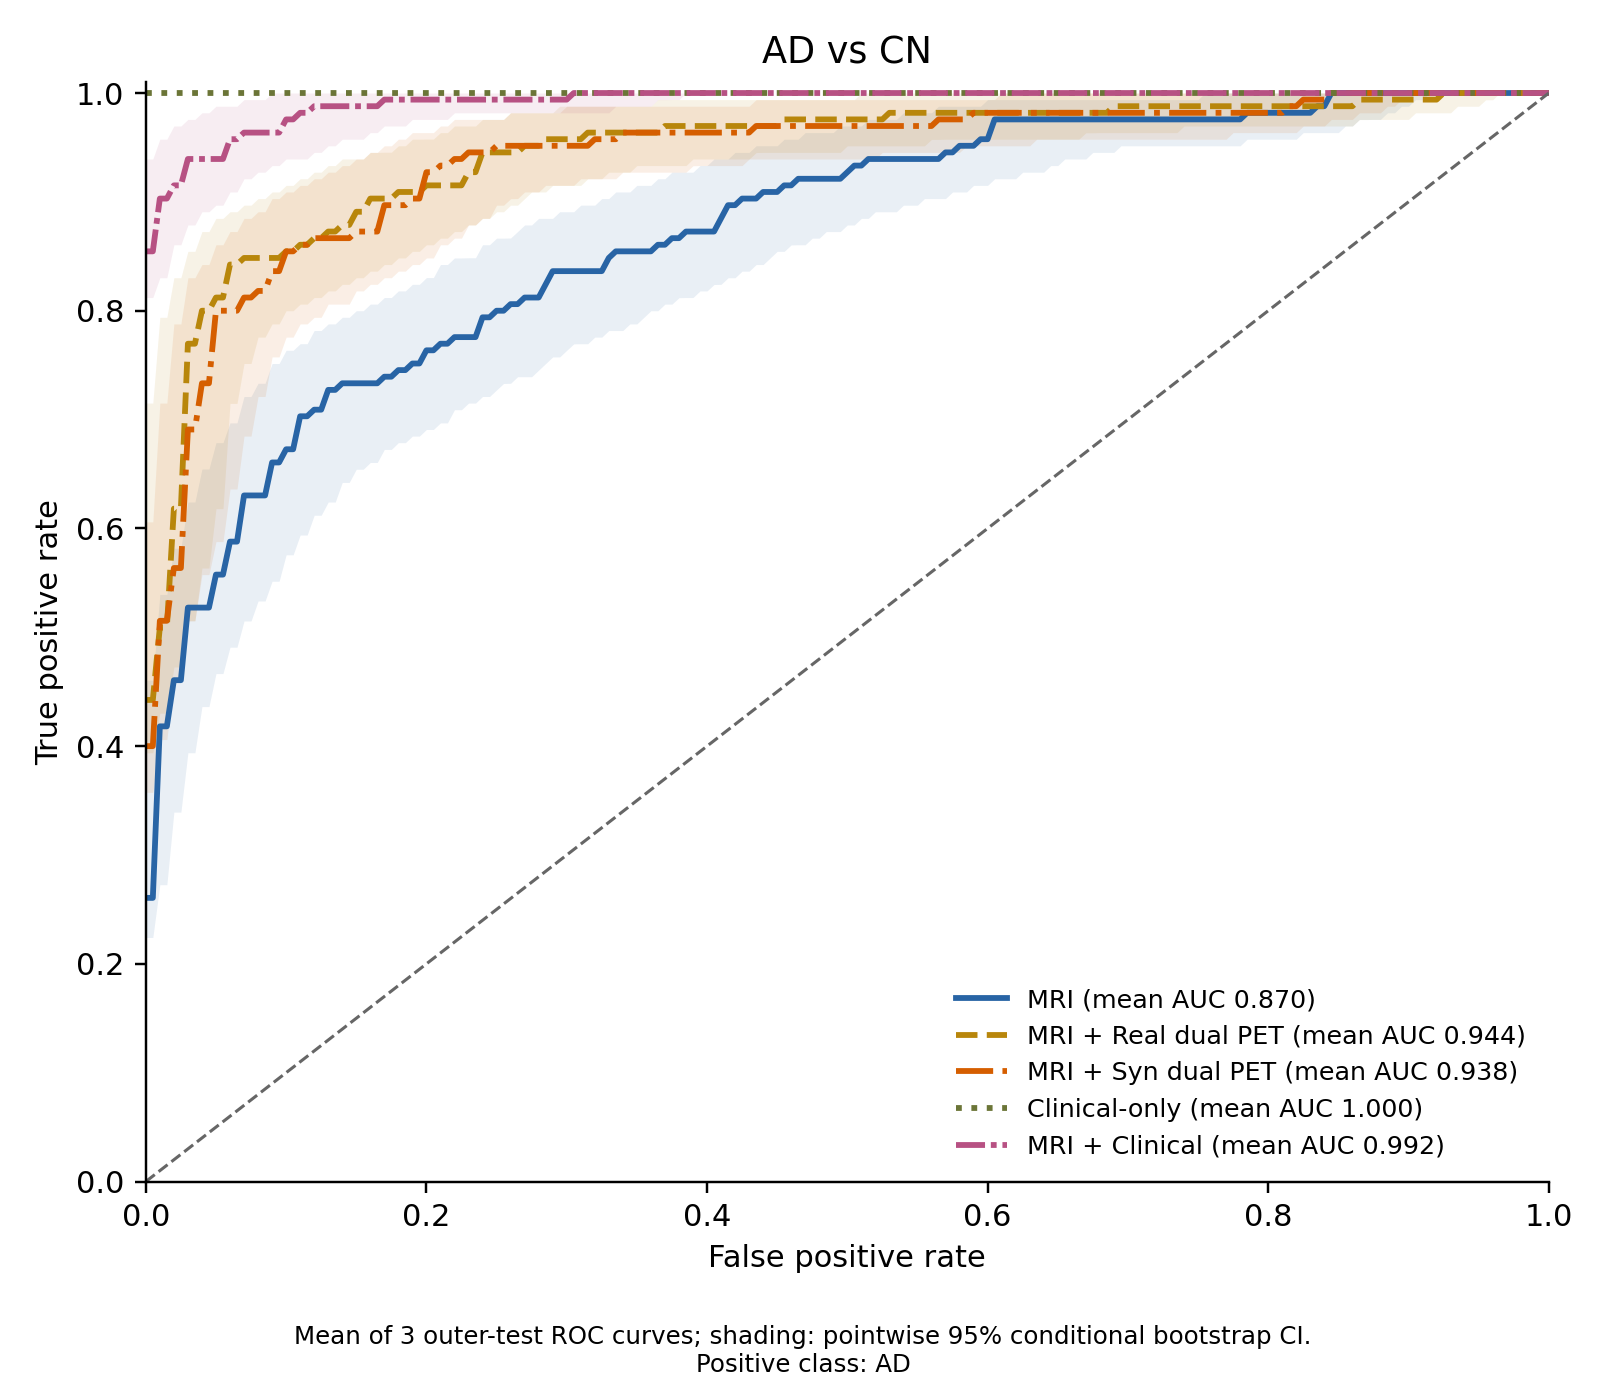
\includegraphics[width=0.32\textwidth]{revision_roc_ad_cn}
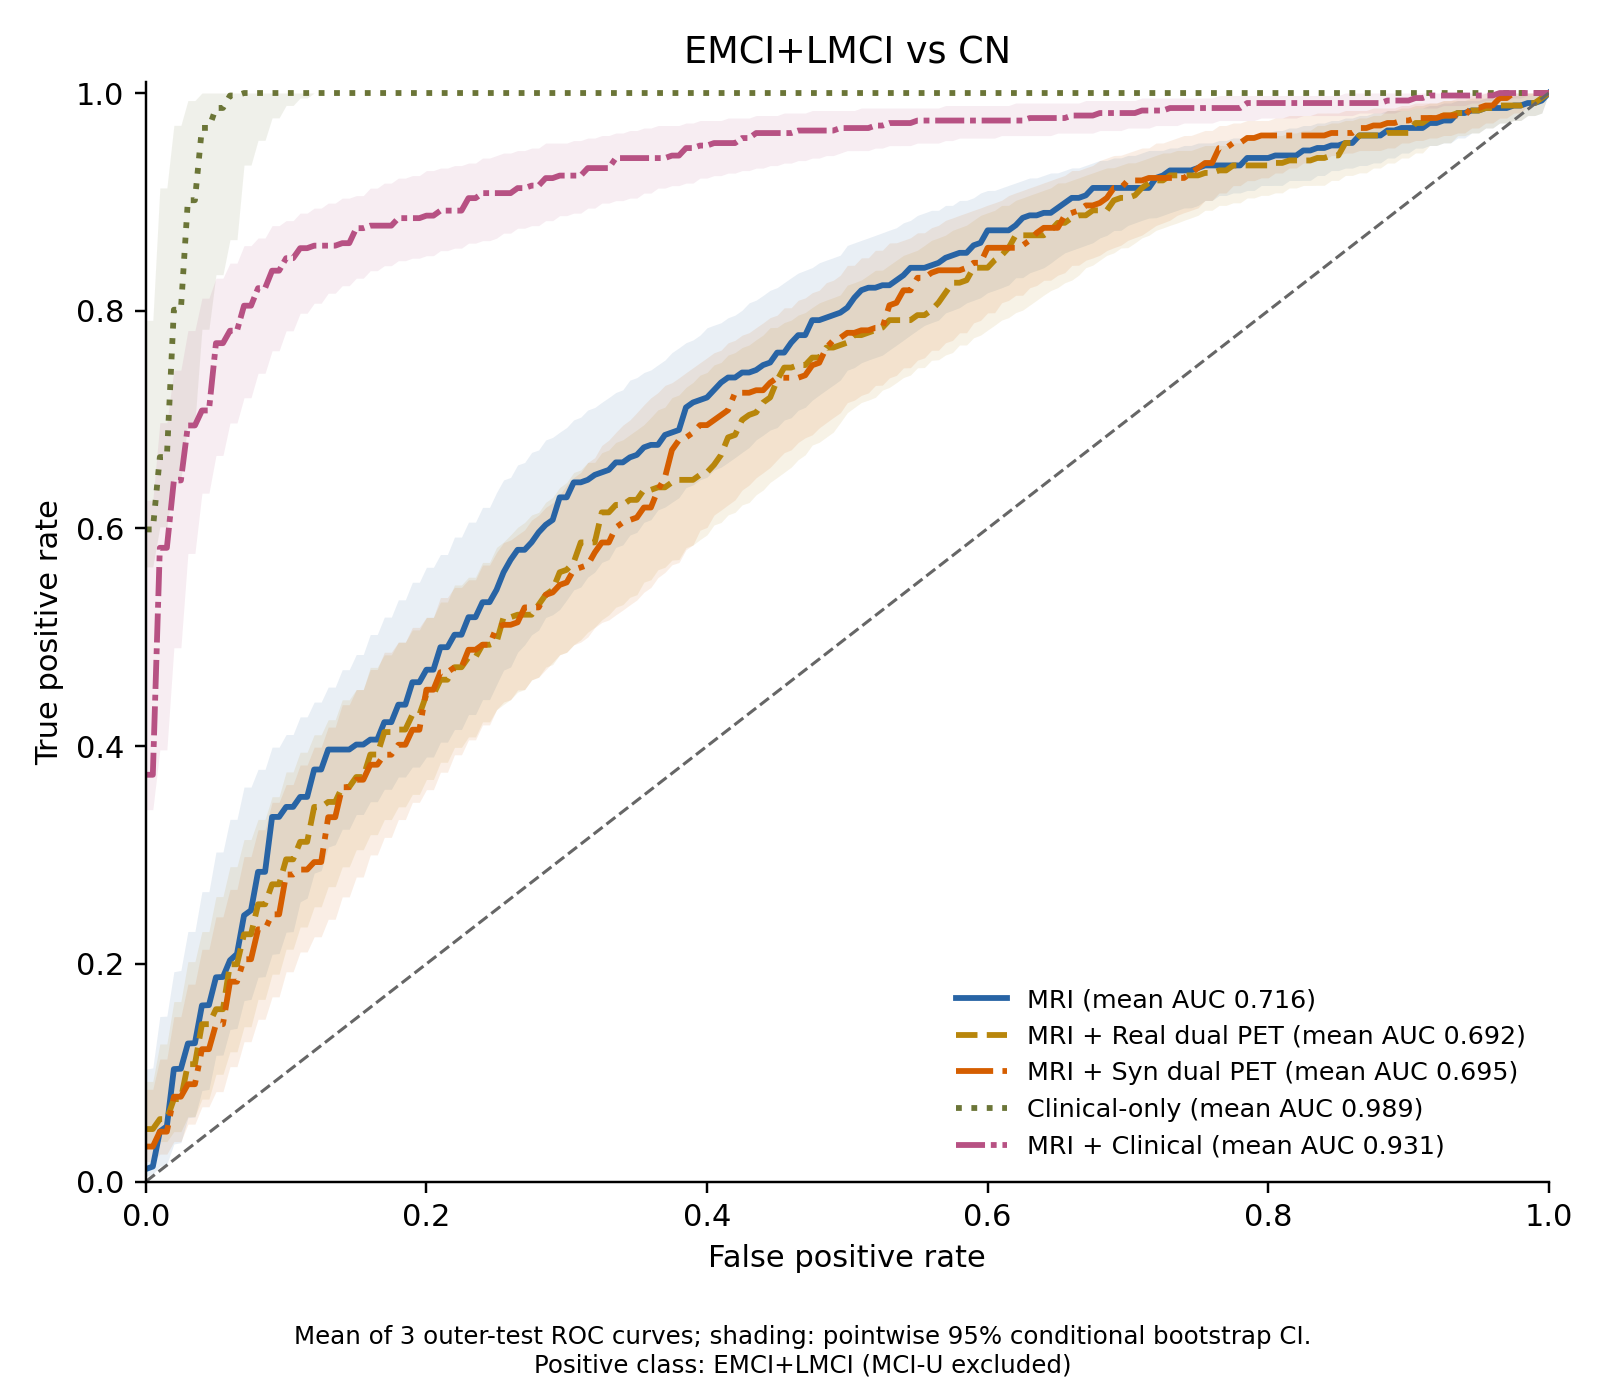
\includegraphics[width=0.32\textwidth]{revision_roc_mci_cn}
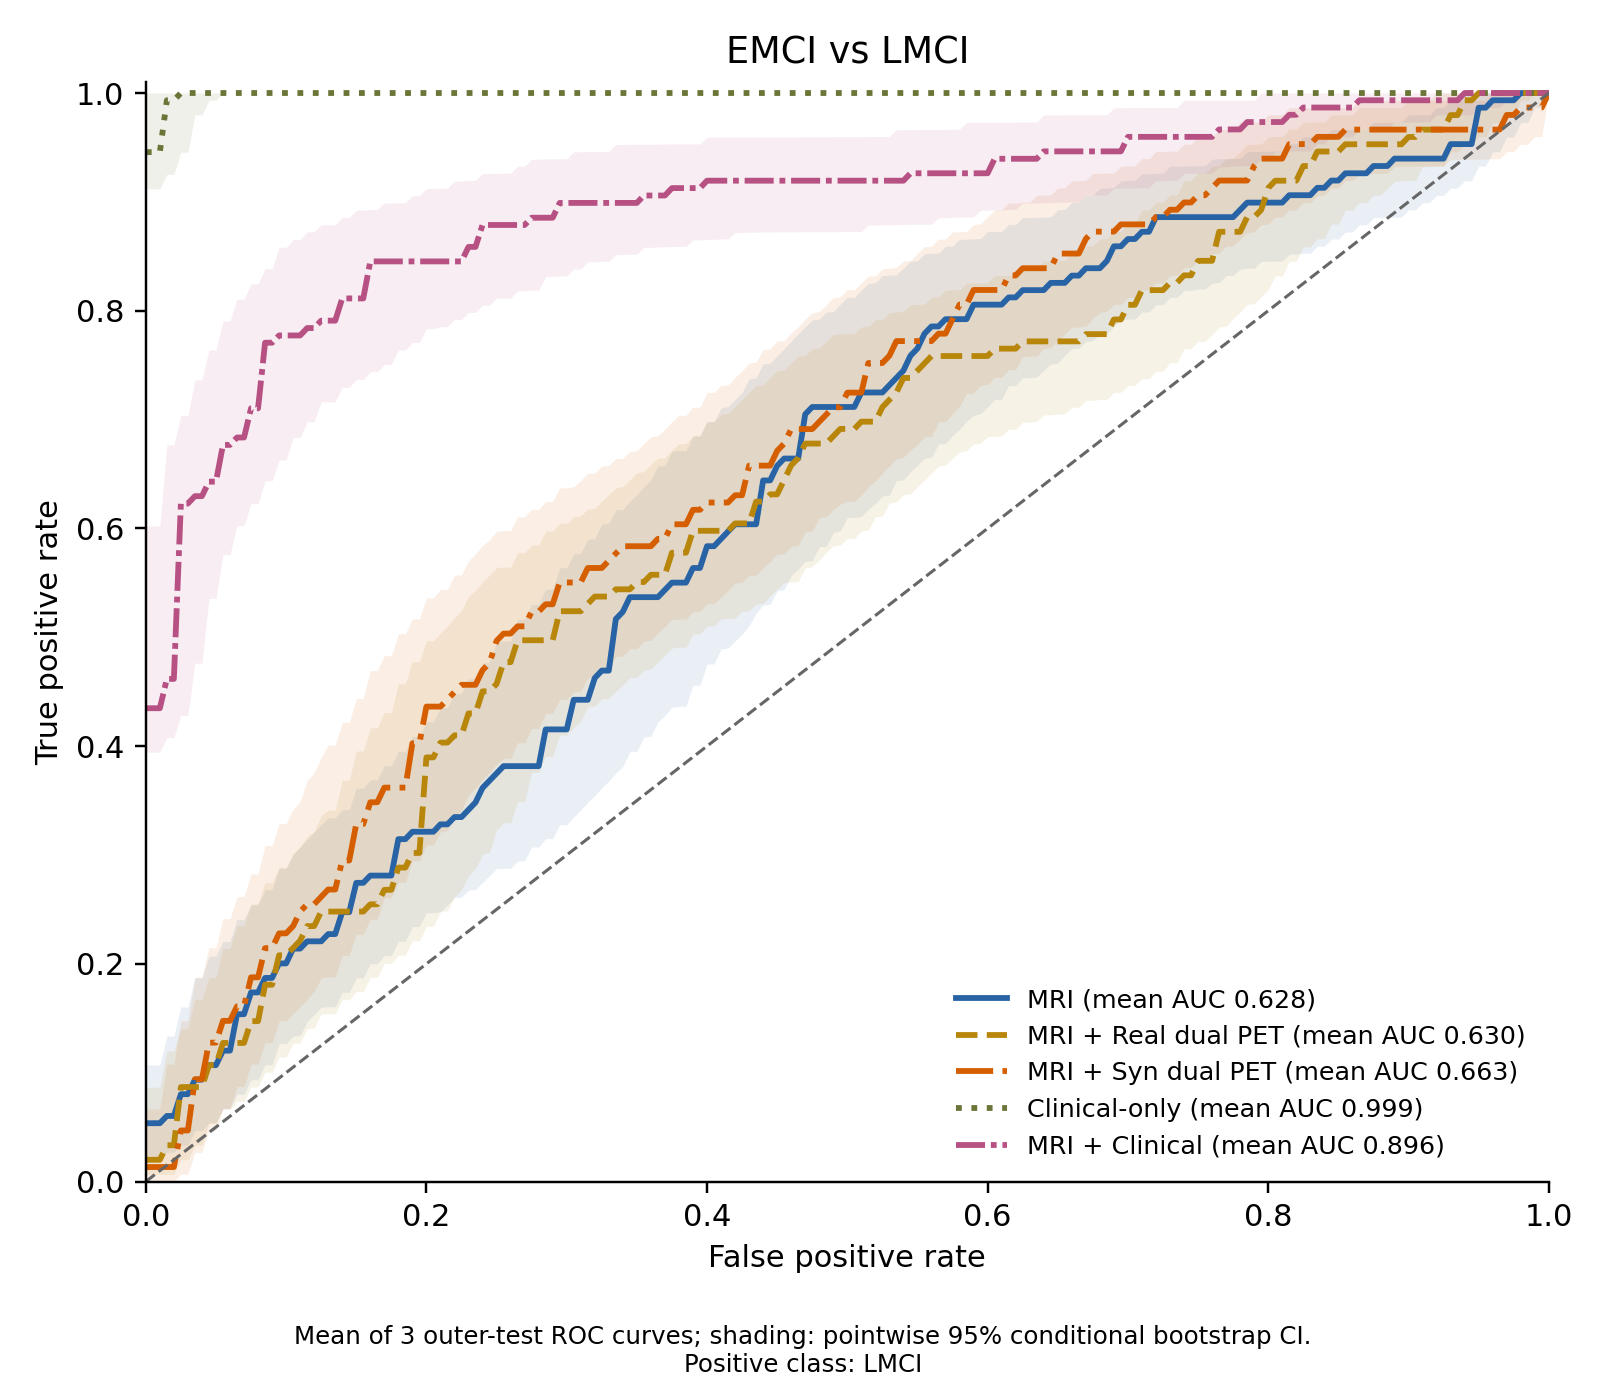
\includegraphics[width=0.32\textwidth]{revision_roc_emci_lmci}
\caption{\textbf{Cross-sectional classification ROC curves for AD/CN, EMCI+LMCI/CN and EMCI/LMCI (left to right).} Curves average three fold-specific TPRs at a fixed FPR grid; shaded regions are pointwise conditional 95\% bootstrap bands, not simultaneous confidence bands. Legend AUC values are equally weighted empirical fold AUC means. Comparisons include MRI, MRI+Real both, MRI+Syn both, Clinical-only and MRI+Clinical. The clinical fields include diagnosis-related scores and historical group-conditioned fills; high clinical AUC is not evidence of independent synthetic-PET benefit.}
\label{fig:classification_roc}
\end{figure}
